
\subsection{Distribution: Marcenko-Pastur, $\gamma = 0.5$}

\begin{figure}[H]
    \centering
    \includegraphics[width=0.85\textwidth]{{SI_figures/Marcenko-Pastur, gamma=0.5/hist}}
    \caption{Experiment: {\bf Hist}}
\end{figure}

\begin{figure}[H]
    \centering
    \includegraphics[width=0.85\textwidth]{{SI_figures/Marcenko-Pastur, gamma=0.5/R0vsR1}}
    \caption{Experiment: {\bf R0-vs-R1}}
\end{figure}

\begin{figure}[H]
    \centering
    \includegraphics[width=0.85\textwidth]{{SI_figures/Marcenko-Pastur, gamma=0.5/SEvsASE}}
    \caption{Experiment: {\bf SE-vs-ASE}}
\end{figure}

\begin{figure}[H]
    \centering
    \includegraphics[width=0.85\textwidth]{{SI_figures/Marcenko-Pastur, gamma=0.5/oracleAttainment}}
    \caption{Experiment: {\bf OracleAttainment}}
\end{figure}

\begin{figure}[H]
    \centering
    \includegraphics[width=0.85\textwidth]{{SI_figures/Marcenko-Pastur, gamma=0.5/regret}}
    \caption{Experiment: {\bf Regret}}
\end{figure}

\begin{figure}[H]
    \centering
    \includegraphics[width=0.85\textwidth]{{SI_figures/Marcenko-Pastur, gamma=0.5/convergenceRate}}
    \caption{Experiment: {\bf ConvergenceRate}}
\end{figure}



\subsection{Distribution: Marcenko-Pastur, $\gamma = 1.0$}

\begin{figure}[H]
    \centering
    \includegraphics[width=0.85\textwidth]{{SI_figures/Marcenko-Pastur, gamma=1.0/hist}}
    \caption{Experiment: {\bf Hist}}
\end{figure}

\begin{figure}[H]
    \centering
    \includegraphics[width=0.85\textwidth]{{SI_figures/Marcenko-Pastur, gamma=1.0/R0vsR1}}
    \caption{Experiment: {\bf R0-vs-R1}}
\end{figure}

\begin{figure}[H]
    \centering
    \includegraphics[width=0.85\textwidth]{{SI_figures/Marcenko-Pastur, gamma=1.0/SEvsASE}}
    \caption{Experiment: {\bf SE-vs-ASE}}
\end{figure}

\begin{figure}[H]
    \centering
    \includegraphics[width=0.85\textwidth]{{SI_figures/Marcenko-Pastur, gamma=1.0/oracleAttainment}}
    \caption{Experiment: {\bf OracleAttainment}}
\end{figure}

\begin{figure}[H]
    \centering
    \includegraphics[width=0.85\textwidth]{{SI_figures/Marcenko-Pastur, gamma=1.0/regret}}
    \caption{Experiment: {\bf Regret}}
\end{figure}

\begin{figure}[H]
    \centering
    \includegraphics[width=0.85\textwidth]{{SI_figures/Marcenko-Pastur, gamma=1.0/convergenceRate}}
    \caption{Experiment: {\bf ConvergenceRate}}
\end{figure}



\subsection{Distribution: Chi10, $\gamma = 0.5$}

\begin{figure}[H]
    \centering
    \includegraphics[width=0.85\textwidth]{{SI_figures/Chi10, gamma=0.5/hist}}
    \caption{Experiment: {\bf Hist}}
\end{figure}

\begin{figure}[H]
    \centering
    \includegraphics[width=0.85\textwidth]{{SI_figures/Chi10, gamma=0.5/R0vsR1}}
    \caption{Experiment: {\bf R0-vs-R1}}
\end{figure}

\begin{figure}[H]
    \centering
    \includegraphics[width=0.85\textwidth]{{SI_figures/Chi10, gamma=0.5/SEvsASE}}
    \caption{Experiment: {\bf SE-vs-ASE}}
\end{figure}

\begin{figure}[H]
    \centering
    \includegraphics[width=0.85\textwidth]{{SI_figures/Chi10, gamma=0.5/oracleAttainment}}
    \caption{Experiment: {\bf OracleAttainment}}
\end{figure}

\begin{figure}[H]
    \centering
    \includegraphics[width=0.85\textwidth]{{SI_figures/Chi10, gamma=0.5/regret}}
    \caption{Experiment: {\bf Regret}}
\end{figure}

\begin{figure}[H]
    \centering
    \includegraphics[width=0.85\textwidth]{{SI_figures/Chi10, gamma=0.5/convergenceRate}}
    \caption{Experiment: {\bf ConvergenceRate}}
\end{figure}



\subsection{Distribution: Chi10, $\gamma = 1.0$}

\begin{figure}[H]
    \centering
    \includegraphics[width=0.85\textwidth]{{SI_figures/Chi10, gamma=1.0/hist}}
    \caption{Experiment: {\bf Hist}}
\end{figure}

\begin{figure}[H]
    \centering
    \includegraphics[width=0.85\textwidth]{{SI_figures/Chi10, gamma=1.0/R0vsR1}}
    \caption{Experiment: {\bf R0-vs-R1}}
\end{figure}

\begin{figure}[H]
    \centering
    \includegraphics[width=0.85\textwidth]{{SI_figures/Chi10, gamma=1.0/SEvsASE}}
    \caption{Experiment: {\bf SE-vs-ASE}}
\end{figure}

\begin{figure}[H]
    \centering
    \includegraphics[width=0.85\textwidth]{{SI_figures/Chi10, gamma=1.0/oracleAttainment}}
    \caption{Experiment: {\bf OracleAttainment}}
\end{figure}

\begin{figure}[H]
    \centering
    \includegraphics[width=0.85\textwidth]{{SI_figures/Chi10, gamma=1.0/regret}}
    \caption{Experiment: {\bf Regret}}
\end{figure}

\begin{figure}[H]
    \centering
    \includegraphics[width=0.85\textwidth]{{SI_figures/Chi10, gamma=1.0/convergenceRate}}
    \caption{Experiment: {\bf ConvergenceRate}}
\end{figure}


